\documentclass[aip,rsi,preprint,graphicx]{revtex4-1}
\usepackage{graphicx}  % needed for figures
\usepackage{dcolumn}   % needed for some tables
\usepackage{bm}           % for math
\usepackage{amssymb} % for math
\usepackage{amsmath} % for math
\usepackage{hyperref} % for links

% avoids incorrect hyphenation
\hyphenation{FPGAs}

\begin{document}

\title{NIST digital servo manual}

\author{David~R.~Leibrandt}
\email{david.leibrandt@nist.gov}
\affiliation{National Institute of Standards and Technology\\325 Broadway St.~Boulder, CO 80305\\USA}

\date{\today}

\maketitle

\tableofcontents

%%%%%%%%%%%%%%%%%%%%%%%%%%%%%%%%%%%%%%%%%%%%%%%%%%
\section{Introduction}
%%%%%%%%%%%%%%%%%%%%%%%%%%%%%%%%%%%%%%%%%%%%%%%%%%

The NIST digital servo is designed to be a general purpose feedback controller, implemented digitally using an FPGA.  The advantages of an all-digital approach include fast and easy (no soldering) reconfiguration of the feedback transfer function, loop shapes that go beyond PID, the ability to perform automatic lock acquisition, and the integration of diagnostics for easy analysis of open and closed loop system performance.  The NIST digital servo has been optimized for feedback control of lasers in atomic, molecular, and optical (AMO) physics experiments, but it should be applicable in other control applications with similar bandwidth, noise, and loop shape requirements.  The key specifications (of hardware V1.0) are are:
\begin{itemize}
\item 1 FPGA (Xilinx Spartan 6 LX150)
\item 2 fast analog input channels (LTC2195, 16 bit, 100 MSPS, 50~nV$/\sqrt{\textrm{Hz}}$)
\item 2 fast analog output channels (AD9783, 16 bit, 100 MSPS, 40~nV$/\sqrt{\textrm{Hz}}$)
\item 1 slow analog output channel (AD5791, 20 bit, 1 MSPS, 20~nV$/\sqrt{\textrm{Hz}}$, optionally amplified to 0V to +65V output range for direct drive of PZTs)
\item Several digital I/O channels
\item 320 ns analog latency (ADC, digital signal processing, and DAC) including a digital PI filter
\item USB communication and GUI for setup and diagnostics
\end{itemize}

This manual describes assembly, setup, and operation of the NIST digital servo.  Section~\ref{sec:quickStart} describes how to assemble the hardware, load the firmware, and install the GUI.  Section~\ref{sec:software} describes how to use the GUI.  For more information about the firmware and performance of the digital servo, as well as example use cases, please read D.~R.~Leibrandt and J.~Heidecker, \href{http://arxiv.org/abs/1508.06319}{arXiv:1508.06319} (2015).

%%%%%%%%%%%%%%%%%%%%%%%%%%%%%%%%%%%%%%%%%%%%%%%%%%
\section{Quick start guide}\label{sec:quickStart}
%%%%%%%%%%%%%%%%%%%%%%%%%%%%%%%%%%%%%%%%%%%%%%%%%%

In order to get started, you will need need:
\begin{itemize}
\item A set of parts to assemble the digital servo hardware box (see \\{\tt digital-servo\textbackslash hardware\textbackslash Enclosure\textbackslash Enclosure\_BOM.xlsx})
\item A low voltage power supply (+5~V, $\pm$12~V; the hardware has been tested successfully with ASTEC model DPT52)
\item A high voltage power supply (up to +68~V; the hardware has been tested successfully with PHIHONG USA model PSAC30U-560)
\item A USB cable
\item A computer (this manual will assume use of the Windows 7 operating system, but we have also compiled and run the digital servo using Linux)
\item Copies of the following software
\begin{itemize}
\item The digital servo GUI and the Qt, Qwt, and Opal Kelly libraries
\item The Opal Kelly USB communication driver
\end{itemize}
\end{itemize}

\subsection{Hardware assembly}

The hardware consists of an Opal Kelly XEM6010-LX150 FPGA evaluation board and a custom daughterboard, packaged together with some fans, some LEDs, and a switch in an enclosure.  Here we assume that the daughterboard has already been fabricated and stuffed, which can be done by a PCB assembly company.  To assemble the digital servo hardware, follow these steps:

\begin{enumerate}
\item Install the connectors, LEDs, fans, and switch onto enclosure front and back panels and wire them up, following Fig.~\ref{fig:DigitalServoInsidePic}
\item Double check that one of the fans blows air into the box and the other blows air out of the box
\item Remove FB2 from the XEM6010-LX150
\item Add the heat sink to the FPGA
\item Press XEM6010-LX150 and the daughterboard together
\item Attach the daughterboard to the enclosure bottom using nylon washers on top so that the screws do not stick out bottom of the box
\item Put the enclosure together and connect the wires
\end{enumerate}

\begin{figure*}
\begin{center}
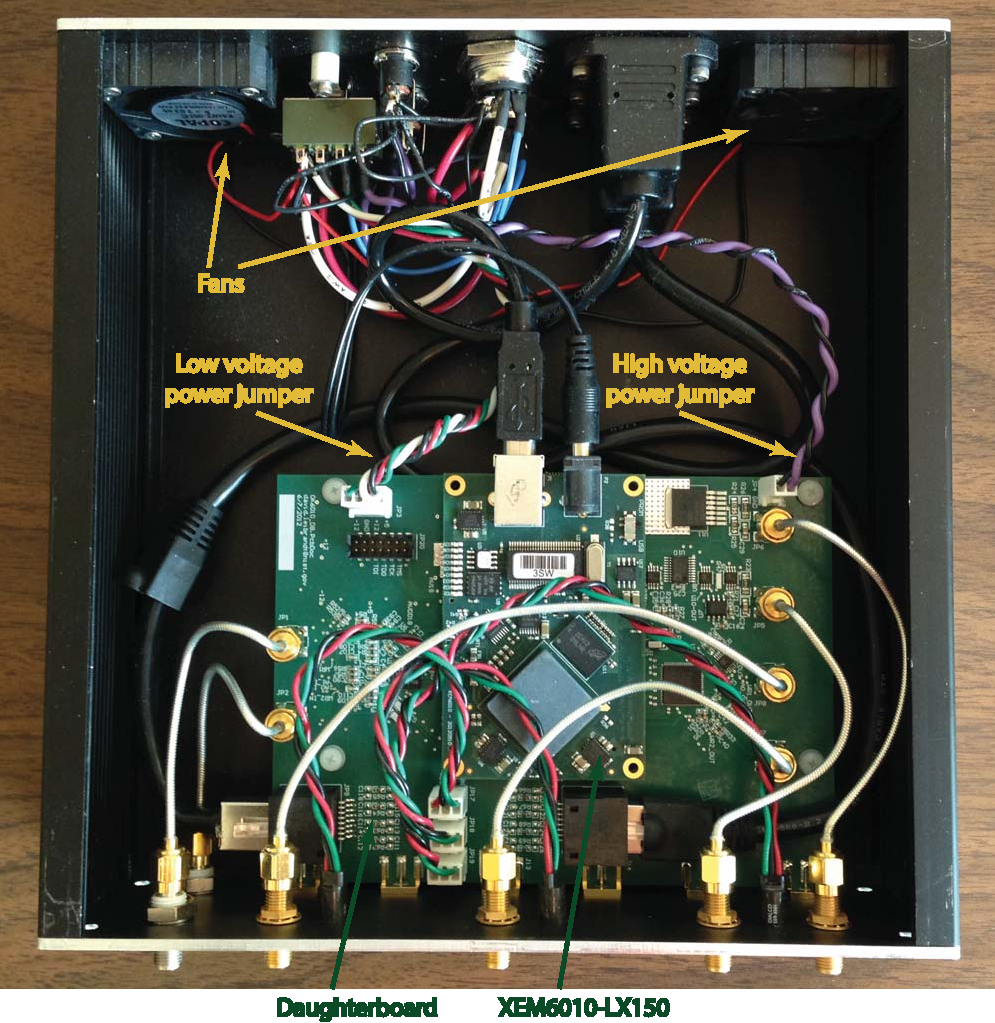
\includegraphics[width=1.0\textwidth]{Figs/DigitalServoInsideWithLabels}
\caption{\label{fig:DigitalServoInsidePic}Picture of the inside of an assembled NIST digital servo box.}
\end{center}
\end{figure*}

When assembly is complete, the hardware box should look like that shown in Fig.~\ref{fig:DigitalServoOutsidePic}.

\begin{figure*}
\begin{center}
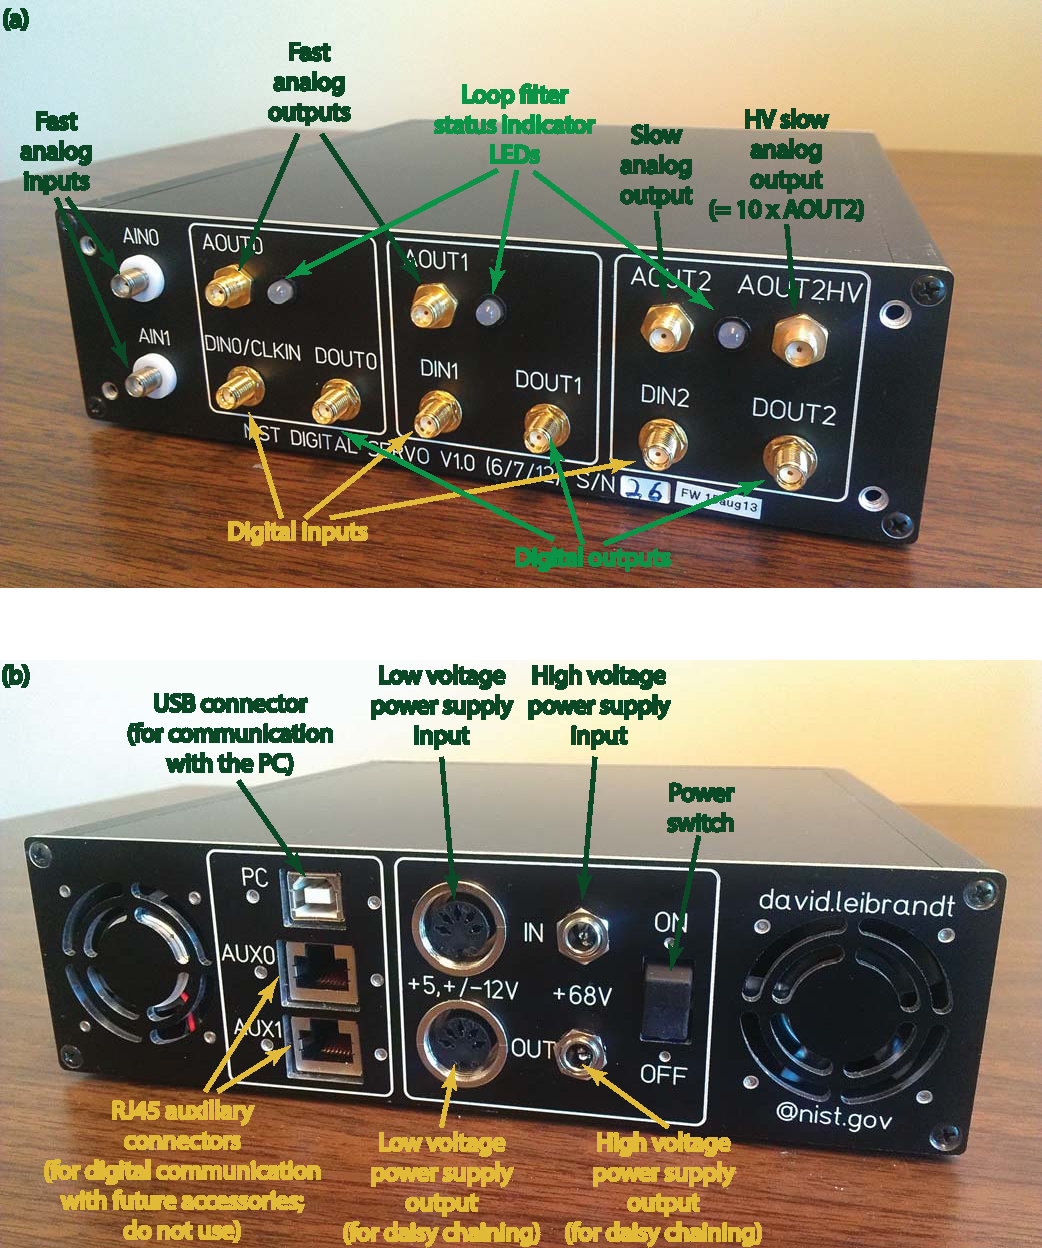
\includegraphics[width=1.0\textwidth]{Figs/DigitalServoOutsideWithLabels}
\caption{\label{fig:DigitalServoOutsidePic}Pictures of the (a) front and (b) back of a NIST digital servo box.  Inputs and outputs are labeled.}
\end{center}
\end{figure*}

\subsection{Loading the firmware}\label{sec:loadFirmware}

The firmware is stored in a FLASH memory on the XEM6010-LX150 and loaded automatically upon turning on the power, so these steps will only need to be executed once after the box is built to load the firmware into the FLASH.  To load the firmware, you will need to use the program flashloader.exe, which ships with the XEM6010-LX150.  Follow these steps:

\begin{enumerate}
\item Install the Opal Kelly communication driver on your computer by running the executable {\tt Setup-Win-Win32-4.0.8.exe} (located in the folder {\tt Opal\_Kelly\_2012\_02\_07} on the Opal Kelly CD) and follow the instructions.
\item Copy flashloader.exe (located in the \\{\tt C:\textbackslash Program~Files\textbackslash Opal~Kelly\textbackslash FrontPanelUSB\textbackslash Samples\textbackslash FlashLoader} folder) and flashloader.bit (located on the Opal Kelly CD in the \\{\tt Opal\_Kelly\_2012\_02\_07\textbackslash Bitfiles\textbackslash 20111007-FP40-XEM6010-LX150.zip\textbackslash XEM6010-LX150} folder) to the \\{\tt digital-servo\textbackslash deploy\textbackslash Windows7\_FW28may15} folder.  
\item Unplug all other digital servo boxes from the computer so that flashloader.exe will select the correct box for for programming.
\item Plug in the digital servo power and USB connections and flip the dip switch on the XEM6010-LX150 to ``USB'' (you will have to open the digital servo enclosure), then flip the power switch to the on position.
\item Open a command prompt (search for ``cmd'' in the Start Menu) and navigate to the \\{\tt digital-servo\textbackslash deploy\textbackslash Windows7\_FW28may15} folder.
\item Execute \\{\tt flashloader.exe superlaserland\_HW07jun12\_CONFIG\_SIMPLEPI\_FW28may15.bit}
\item Flip the dip switch on the XEM6010-LX150 to ``PROM'', then power cycle the digital servo and close up the enclosure.
\end{enumerate}

\subsection{Installing the software}\label{sec:installSoftware}

Follow these steps to install the GUI:

\begin{enumerate}
\item If you have not already done so on this computer, install the Opal Kelly communication driver (see Section~\ref{sec:loadFirmware}, step 1).
\item Copy okFrontPanel.dll (located in the \\{\tt C:\textbackslash Program~Files\textbackslash Opal~Kelly\textbackslash FrontPanelUSB\textbackslash API-32} folder) to the \\{\tt digital-servo\textbackslash deploy\textbackslash Windows7\_FW28may15} folder.
\item Create an empty folder {\tt C:\textbackslash data\textbackslash SuperLaserLand}.  This is the location where any data saved by the digital servo can be found.
\item Connect the low voltage and high voltage power supplies.  Note that there are two connectors for each power supply on the back of the digital servo box.  This is to allow running up to four digital servo boxes on a single pair of power supplies, using daisy chain cables.  Also note that if you do not intend to use the high voltage output (AOUT2HV), you do not need the high voltage power supply.
\item Ensure that the power switch on the back of the digital servo is in the off position, then connect the USB cable to the back of the digital servo box and to your PC.
\item Flip the power switch on the back of the digital servo to the on position and wait 15~s for the FPGA to initialize.
\item Run the executable {\tt SuperLaserLand\_FW28may15.exe} and you should be ready to go!  See Sec.~\ref{sec:software} for a description of how to use the GUI.
\end{enumerate}

%%%%%%%%%%%%%%%%%%%%%%%%%%%%%%%%%%%%%%%%%%%%%%%%%%
\section{Graphical user interface}\label{sec:software}
%%%%%%%%%%%%%%%%%%%%%%%%%%%%%%%%%%%%%%%%%%%%%%%%%%

Communication between the NIST digital servo hardware and the computer is facilitated by a GUI program called SuperLaserLand (see Fig.~\ref{fig:SoftwareScreenshot}).  Follow the instructions found in Sec.~\ref{sec:installSoftware} in order to launch SuperLaserLand.

\begin{figure*}
\begin{center}
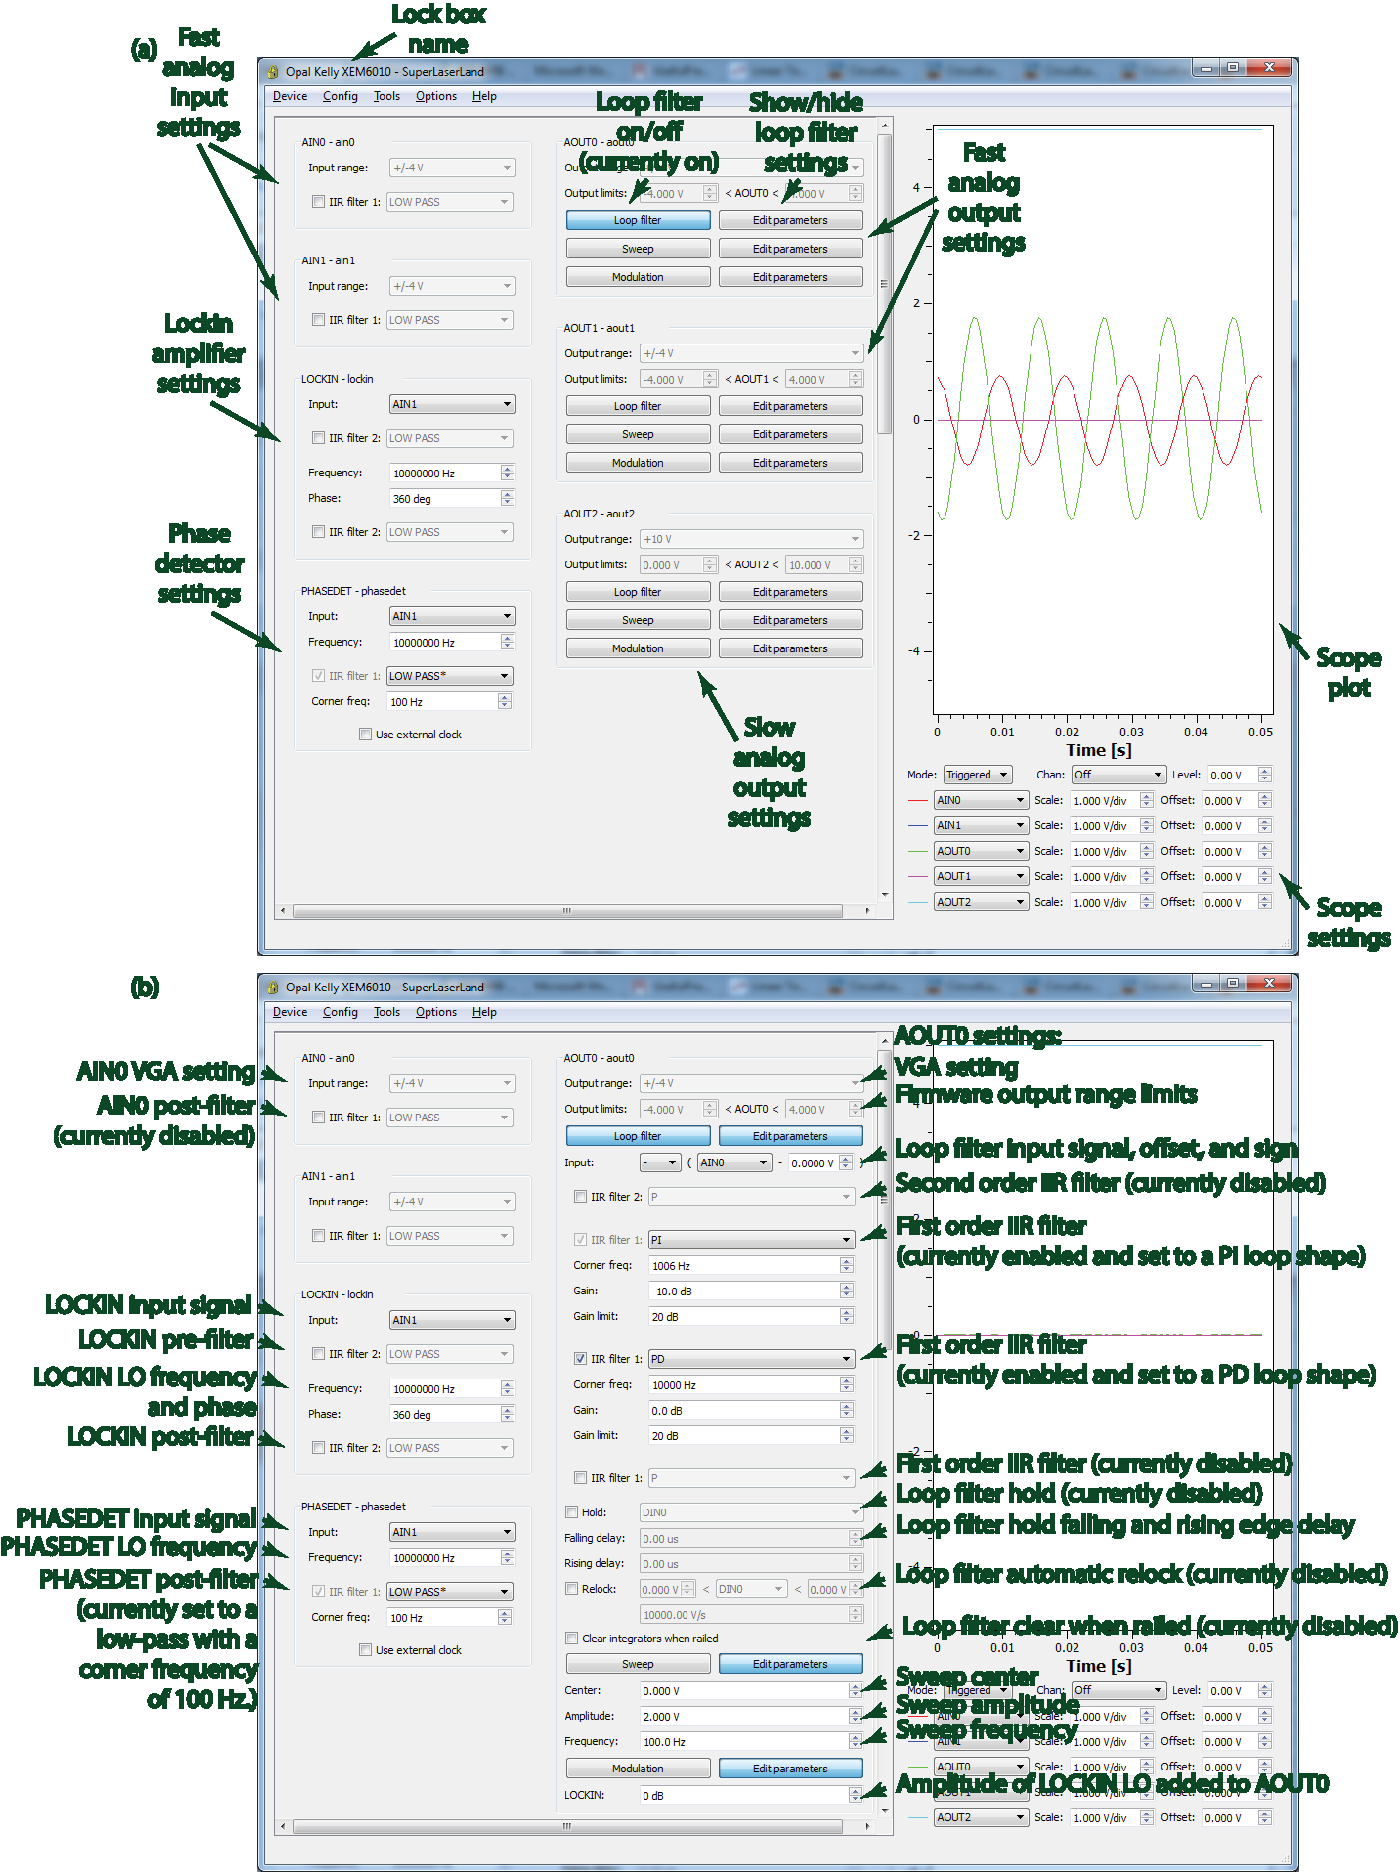
\includegraphics[width=1.0\textwidth]{Figs/SuperlaserlandOverview}
\caption{\label{fig:SoftwareScreenshot}Screen shots of the SuperLaserLand GUI.  The settings for the AOUT loop filter, sweep, and modulation can be (a) hidden or (b) shown.  Most of the configuration settings are labeled.}
\end{center}
\end{figure*}

\subsection{{\tt Device} menu}

The {\tt Device} menu contains commands pertaining to the digital servo hardware.  The {\tt Set name} command is used to set the name of the digital servo box.  This name is displayed at the top left of the SuperLaserLand window and is helpful when communicating with multiple digital servo boxes using a single PC.  If the GUI is launched when more than one digital servo box is connected to the computer, the user will be asked to select the hardware box they wish to communicate with by this name.  The {\tt Send command}, {\tt Optimize LTC2195 timing}, and {\tt Optimize AD9783 timing} commands are used for debugging and should not be needed by the typical user.

\subsection{{\tt Config} menu}

The {\tt Config} menu contains commands for saving and loading the digital servo configuration (i.e., digital signal processing settings).  The current configuration can be saved to or loaded from a FLASH memory located in the digital servo box using the {\tt Save to FLASH} or {\tt Load from FLASH} commands.  The FLASH memory can only hold one configuration at a time, so any previously saved configuration is overwritten each time the {\tt Save to FLASH} command is used.  The FLASH memory is nonvolatile, and the configuration saved in the FLASH memory is loaded automatically on power up.  The current configuration can also be saved to or loaded from the PC, using the {\tt Save to file} or {\tt Load from file} commands.  This allows the user to save multiple configuration files and to transfer the configuration from one digital servo to another (via the PC).

\subsection{{\tt Tools} menu}

The {\tt Tools} menu contains commands used for diagnostics of the digital servo and the system under servo control.

The {\tt Record data} command is used to record all of the digital servo signals to a binary file on the PC at a user defined sample rate and for a user defined total number of samples.  The resulting data file can be found in {\tt C:\textbackslash data\textbackslash SuperLaserLand} and is labeled {\tt <TIMESTAMP>.dat}.  It can be read into matlab using the function \\{\tt readSuperLaserLandSimplePI.m} located in the {\tt digital-servo\textbackslash matlab} folder.

The {\tt Measure transfer function} command is used to measure transfer functions.  It temporarily adds a swept sinusoidal modulation to one of the analog outputs.  For each value of the modulation frequency, a data file containing the values of digital servo signals is recorded to the PC (by internally calling the {\tt Record data} command).  The data files can be found in the directory {\tt C:\textbackslash data\textbackslash SuperLaserLand\textbackslash <TIMESTAMP>} and are labeled {\tt <MODULATION FREQ>.dat}.  Data processing to compute the transfer function from the recorded files is performed offline in matlab.

\subsection{{\tt Options} menu}

The {\tt Options} menu contains software options.

The {\tt Edit analog configuration} option must be enabled in order to be able to change the analog input and output ranges.  This prevents the user from accidentally changing the input and output ranges, which in some circumstances may damage the system under servo control.  In addition, when the {\tt Edit analog configuration} option is enabled, the user can change the names of the analog signals by typing a new name in the {\tt Name} text field that appears at the top of the signal box {\it and pressing enter}.  For instance, AIN0 could be renamed ``HC error signal'' and AOUT2 could be named ``PZT''.  These names are saved with the digital servo configuration.

When the {\tt Log data} option is enabled, the digital servo records the values of the analog signals to a text file on the PC at a user defined interval, indefinitely.  At the end of each time interval the minimum, maximum, and mean values of each signal over the time interval are recorded.  The data file can be found in {\tt C:\textbackslash data\textbackslash SuperLaserLand} and is labeled {\tt <TIMESTAMP>.csv}.  It can be read into matlab using the function {\tt readSLLlog.m} located in the {\tt digital-servo\textbackslash matlab} folder.

\subsection{Analog input configuration}

Each analog input has configuration settings located in the {\tt AIN0} and {\tt AIN1} boxes that allow processing of the input signals before they are used for feedback.  The gain of the VGA before the ADC can be set using the {\tt Input range} drop down list, which can only be accessed when the {\tt Edit analog configuration} option is enabled.  In addition, the digitized ADC signal can optionally be filtered by a first order IIR filter.  In order to enable the IIR filter, click the checkbox to the left of the label {\tt IIR filter 1} (which stands for first order IIR filter).  The filter shape can be changed using the drop down list, and the filter parameters can be set using the numerical input boxes below.  For example, when the filter shape is set to {\tt LOW PASS}, the low-pass corner frequency and gain can be adjusted.

\subsection{Lock-in amplifier configuration}

The lock-in amplifier settings are located in the box labeled {\tt LOCKIN}.  From top to bottom the settings are the input signal ({\tt Input} drop down list), the second order IIR pre-filter (top {\tt IIR filter 2}), the LO frequency and demodulation phase, and the second order IIR post-filter (bottom {\tt IIR filter 2}).

\subsection{Phase detector configuration}

The phase detector settings are located in the box labeled {\tt PHASEDET}.  From top to bottom the settings are the input signal ({\tt Input} drop down list), the LO frequency, the first order low-pass IIR filter frequency, and the use external clock setting.  Note that that majority of the FPGA is clocked on an internal crystal oscillator clock, and that the phase detector optionally uses an external clock to clock the local oscillator.  The external clock must be a square wave fed into DIN0, have a low level of 0~V and a high level of 3.3~V, and have a frequency of 10~MHz.

\subsection{Analog output configuration}

The analog output settings are located in the {\tt AOUT0}, {\tt AOUT1}, and {\tt AOUT2} boxes.  The gain of the VGA after the DAC can be set using the {\tt Output range} drop down list and the firmware output range limits can be set using the {\tt Output limits} numerical input boxes.  These settings can only be accessed when the {\tt Edit analog configuration} option is enabled.

Each analog output signal is generated as the sum of a loop filter, a sweep module that generates a triangle wave sweep, and a relock module that performs automatic lock acquisition.

The analog output loop filter can be turned on or off using the {\tt Loop filter} button.  When SuperLaserLand is first opened, the loop filter settings are hidden.  In order to display the loop filter settings, press the {\tt Edit parameters} button to the right of the {\tt Loop filter} button.  The loop filter input can be set to any of the analog signals with an optional constant offset and sign flip.  The loop filter consists of one or more first and second order IIR filters applied sequentially to the input signal.  The settings for these filters are shown from top to bottom in the order the filters are applied, starting with a second order IIR filter ({\tt IIR filter 2}) and followed by one to three first order IIR filters ({\tt IIR filter 1}).  Only the first first-order IIR filter must be enabled; the other IIR filters are optional.  For example, a ``PIID'' loop shape can be configured by disabling the second order IIR filter and enabling the three first order IIR filters, with loop shapes PI, PI, and PD.  Alternatively, an integrator with a notch (appropriate for feedback to a PZT with a resonance) can be configured by enabling the second order IIR filter and the first first-order IIR filter with loop shapes I/HO and P (note that I/HO stands for integrator divided by harmonic oscillator).  Note that the first and second order IIR filters have latencies of 30 and 80 ns.  The latency of each module should be kept in mind when selecting a loop filter configuration for high-bandwidth applications.

An optional loop filter hold feature (``integrator hold'') can be enabled using the checkbox to the left of the label {\tt Hold}.  When this feature is enabled, the output of the loop filter will be constant when the signal selected to the right of the label {\tt Hold} is boolean true.  When DIN0, DIN1, or DIN2 is selected, the loop filter output is held constant when the digital input is TTL high.  When !DIN0, !DIN1, or !DIN2 is selected, the loop filter output is held constant when the digital input is TTL low.  When LOOP FILTER 0, 1, or 2 is selected, the loop filter output is held constant when the other loop filter is unlocked (which is detected only if the relock feature on that loop filter is enabled).  The falling and rising edges of the hold signal can optionally be delayed by independent time intervals, which are set using the {\tt Falling delay} and {\tt Rising delay} input boxes.  This feature is useful, for instance, when performing intensity stabilization of a short laser pulse.

An optional loop filter automatic relock feature can be enabled using the checkbox to the left of the label {\tt Relock}.  To the right of the {\tt Relock} label there is a drop down list that allows the user to select the signal that will determine whether the loop filter is locked or not.  When an analog signal is selected, the loop filter is considered locked when the value of that analog signal is between the user input bounds.  When a digital signal is selected, the loop filter is considered locked when the digital signal is TTL low.  When the loop filter is unlocked, the relock feature sweeps the output of the loop filter in a triangle wave with an amplitude that increases with time and a (constant) user selected slew rate, until lock is reacquired.

Finally, the loop filter output can optionally be reset to zero when it reaches one of the output limits using the checkbox to the left of the label {\tt Clear integrators when railed}.  This feature is useful for locking cavities or interferometers where the error signal is periodic and it does not matter to which fringe the system is locked.

The analog output sweep can be turned on or off using the {\tt Sweep} button, and the sweep settings can be shown by pressing the {\tt Edit parameters} button to the right of the {\tt Sweep} button.  The sweep is a triangle wave, with adjustable offset ({\tt Center} input box), amplitude, and frequency.  In order to DC bias the analog output, turn on the sweep with zero amplitude.

The lock-in amplifier LO can be added to the analog output by pressing the {\tt Modulation} button, and the modulation amplitude can be shown and adjusted by pressing the {\tt Edit parameters} button to the right of the {\tt Modulation} button.

\subsection{Scope configuration}

The right side of the SuperLaserLand GUI contains a basic oscilloscope that can be used to display the digital servo signals in real-time.  The oscilloscope has three modes: Off, Rolling, and Triggered.  When Rolling mode is selected the time base of the scope is 20~s, and when Triggered mode is selected the time base of the scope is 50~ms.  These are not adjustable.  The oscilloscope can display up to five traces simultaneously.  For each trace, the user can select the digital servo signal to be displayed, the vertical scale, and the vertical offset.

\end{document}
%
% ****** End of file template.aps ******
